% Created 2025-03-05 Wed 20:07
% Intended LaTeX compiler: lualatex
\documentclass[10pt]{scrartcl}


\KOMAoptions{
%headings=chapterprefix,
twocolumn=true,
%toc=indenttextentries,
%toc=flat,
twoside=true,
headinclude=true,
footinclude=true
%  captions=topbeside
}
%\usepackage[fontsize=12.3]{scrextend}
\usepackage{fontspec}
\usepackage[T1]{fontenc}
\usepackage[english, portuguese, american]{babel}
\usepackage{hyperref}
\usepackage[x11names,svgnames,table]{xcolor}
\defaultfontfeatures{Ligatures=TeX}
%%\setmainfont{Lato}
%%\setmainfont{Charis SIL}
\setmainfont{IBM Plex Serif}
\usepackage{typearea}
\usepackage{lscape}
\usepackage[a4paper]{geometry}
\geometry{a4paper,total={170mm,257mm},left=10mm,right=10mm, top=15mm, bottom=20mm}
\usepackage[english,portuguese]{babel}
\usepackage{amsmath,amsfonts,amsthm,bm}
\usepackage{graphicx}
\usepackage{float,wrapfig}
\usepackage{colortbl}
\usepackage{tabularx}
\usepackage{pst-labo}
\usepackage{setspace}
\usepackage{xfrac}
\usepackage{tikz}
\usepackage{pgfplots}
\pgfplotsset{compat=1.3}
%% Diagraman latex
\usepackage{endiagram}
\usepackage{smartdiagram}
\usepackage[tikz]{bclogo}
\usetikzlibrary{fit,patterns,shadows.blur,shapes,decorations.pathreplacing,decorations.markings,arrows.meta,arrows,positioning,shadows,trees}
\usetikzlibrary{decorations.pathmorphing} %% to chemfig config bond
\usepackage{upgreek}
\usepackage[modules={all}]{chemmacros}
%%\chemsetup{modules={reactions,spectroscopy,thermodynamics,redox,isotopes}}
%%\chemsetup{modules={all}}
\NewChemState\EPot{ symbol=E , subscript-pos=right , superscript=o, pre= , unit=\volt }
%\usepackage[version=4,arrows=pgf-filled]{mhchem}
\usepackage{chemfig,elements,cancel,siunitx}
\NewChemPhase\lqdd{\(\ell\)}
\NewChemPhase\gr{grafite}
\NewChemPhase\reac{reação}
%\setchemfig{fixed length=false, atom sep=2.0em, arrow offset=6pt, scheme debug=false,angle increment=30}
\setchemfig{angle increment=30, atom sep=1.67em, double bond sep=0.67ex, bond style={line width=0.1em}, cram width=0.8ex, cram dash width=0.1em, cram dash sep=0.2em, arrow style={line width=0.067em},  arrow head=-{Triangle}, arrow label sep=1ex, cycle radius coeff=0.75, chemfig style={line width=0.1em}, }
\renewcommand{\CancelColor}{\color{red}}
\usepackage{circuitikz}
\usepackage{mol2chemfig}
\usepackage{subfig,caption}
\captionsetup{font=small, labelfont={bf,sf}}
\usepackage{wrapfig,qrcode}
\usepackage{array,longtable} % ajust colunm table
\newcolumntype{J}{>{\centering\arraybackslash}m{7.5cm}}
\newcolumntype{K}{>{\centering\arraybackslash}m{6.5cm}}
\newcolumntype{L}{>{\centering\arraybackslash}m{5cm}}
\newcolumntype{B}{>{\centering\arraybackslash}m{2.5cm}}
\newcolumntype{N}{>{\centering\arraybackslash}m{1.4cm}}
\usepackage[most]{tcolorbox}
\newcounter{mycounter}
%%% Colobor
%%% Example colorbox
\newtcolorbox{Box2}[2][]{
lower separated=false,
colback=white,
colframe=black,fonttitle=\bfseries,
colbacktitle=black,
coltitle=white,
enhanced, attach boxed title to top left={yshift=-0.1in,xshift=0.15in}, boxed title style={boxrule=0pt,colframe=white,}, title=#2,#1}
%%%%%%%% Cabecalho
\usepackage{framed,amsmath}
\newtcolorbox{mybox}[2][]{
enhanced,title=#2, fonttitle=\sffamily\small,
top=2pt,
bottom=1mm,
boxrule=0.4pt,
coltitle=black,
colback=white,
attach boxed title to top center={yshift=-\tcboxedtitleheight/2,
yshifttext=-\tcboxedtitleheight/2},
boxed title style={
colframe=white,
colback=white,
left=0.2pt,
right=0.2pt},
#1}
\usepackage{tabularray}
%%%%%%
\newtcolorbox{exercisebox}%
{enhanced,breakable,colback=white, colframe=green!15!white,colbacktitle=white!15!pink, coltitle=pink!50!black,left=0pt,right=0mm,top=3mm,bottom=3mm,pad at break=0pt,bottomrule at break=0pt,toprule at break=0pt,borderline={0mm}{0mm}{green!50!white,dashed}, attach boxed title to top center={yshift=-2mm},boxed title style={boxrule=0.4pt},title=Exercícios,}
\usepackage{eso-pic}
\usepackage{etoolbox}
\usepackage{enumitem}
\newcommand\circitem[1]{%
\tikz[baseline=(char.base)]{%https://tex.stackexchange.com/questions/204116/uniform-size-of-circles-around-enumitems
\node[circle,draw=gray, fill=gray!30,
minimum size=1.2em,inner sep=0] (char) {#1};}}
\newcommand\boxitem[1]{%
\tikz[baseline=(char.base)]{%https://tex.stackexchange.com/questions/204116/uniform-size-of-circles-around-enumitems
\node[fill=orange!30,
minimum size=1.2em,inner sep=0] (char) {#1};}}
%\usepackage{widetext}% needs packages "flushend" & "cuted" of "sttools" % bundle, which perhaps must separately be installed
\newcommand{\dd}[1]{\hspace{2pt}d#1}
\definecolor{color1}{RGB}{0,0,90} % Color of the article title and sections
\definecolor{color2}{RGB}{0,20,20} % Color of the boxes behind the abstract and
\definecolor{cinza}{HTML}{C0C0C0}
%%% Custom Exercios
\usepackage{bohr}
\usepackage{multicol}
\setlength{\columnsep}{1.5cm}
\setlength{\columnseprule}{0.2pt}
\usepackage[no-files]{xsim}
\usepackage{tasks}
\xsimsetup{
goal-print={\pgfmathprintnumber[fixed zerofill,precision=1]{#1}}
}
\newcommand*\circled[2]{\tikz[baseline=(char.base)]{
\node[shape=circle,fill,inner sep=2pt, text=white] (char) {#1};}}
%%%%%-Custom Xsim exercises %%%%%
\DeclareExerciseEnvironmentTemplate{custom}
{%\item[\GetExerciseProperty{counter}]
\Needspace*{0\baselineskip}
\noindent
\circled{\XSIMmixedcase{\GetExerciseProperty{counter}}}~~~%
\noindent
\IfInsideSolutionF{%
\GetExercisePropertyT{points}{ % notice the space
(%
\printgoal{\PropertyValue}
\IfExerciseGoalSingularTF{points}
{%\XSIMtranslate{point}
}
{% \XSIMtranslate{points}
}%
)%
}
}}
{\vspace{\baselineskip}}
%%%%%------- Custom  resposta -------%%%%%%%
\DeclareExerciseEnvironmentTemplate{space}
%{\textbf{\GetExerciseProperty{counter}} }
{\noindent\circled{\XSIMmixedcase{\GetExerciseProperty{counter}}}~~~}
% {\circled{\XSIMmixedcase{\GetExerciseProperty{counter}}}}~~~%
{\qquad}
\newcommand*\answer[1]{%
\XSIMexpandcode{%
\SetExerciseProperty{solution-body}
{\noexpand{\Alph{task}}}}%
#1%
}
%\sisetup{locale=DE}
\xsimsetup{
collect = true,
exercise/within = section,
exercise/template = custom,
exercise/the-counter =  \arabic{exercise},
solution/template= custom ,
%%solution-name = solution,  % used with headings=true
%solution/print=true,
%print-collection/print=both,
%print-solutions/collection=true
%goal-print= {\pgfmathprintnumber[fixed zerofill,precision=1]\num{#1}}
}
\RenewDocumentCommand\printpoints{}{%
\TotalExerciseTypeGoal{exercise}{points}{}{}%
}
\NewTasksEnvironment[label = (\emph{\alph*}), label-width = 12pt]{choice}[\choice]
\newenvironment{questions}{\itemize}{\enditemize}
\everymath{\displaystyle}
\DeclareExerciseHeadingTemplate{solution}{%
\section*{Gabarito}%
}
%\usepackage{filecontents}
\NewTblrTheme{fancy}{
\SetTblrStyle{firsthead}{font=\bfseries}
\SetTblrStyle{firstfoot}{fg=blue2}
\SetTblrStyle{middlefoot}{\itshape}
\SetTblrStyle{caption-tag}{red2}
}

\newcommand{\lh}{\underline{\hspace{1cm}}}
%%\onehalfspacing
\def\professor{Fábio Lima}
\def\aluno{ }
\def\numerochamada{}
\def\disciplina{Química}
%%\def\disciplina{UC III}
%%\def\disciplina{R.A.}
\def\turma{}
\def\tipo{{\bfseries Avaliação Bimestral}}
%%\def\tipo{\bfseries Avaliação Mensal}
\def\tipo{\bfseries Exame Final}
\def\bimestre{4 Bimestre}
\def\escola{E.E. 26 de Agosto}
%\def\escola{E.E. José Mamede de Aquino}
%\def\escola{E.E. Joaquim Murtinho}
\def\dataprova{}
\date{\today}
\title{}
\hypersetup{
 pdfauthor={},
 pdftitle={},
 pdfkeywords={},
 pdfsubject={},
 pdfcreator={Emacs 29.4 (Org mode 9.6.15)}, 
 pdflang={English}}
\begin{document}

\selectlanguage{portuguese}
\twocolumn[
\input{../Modelos/CabeOficial}
%\input{../Modelos/cabenovo}
%\input{../Modelos/mamede}
%\input{../Modelos/26agosto}
%% \input{../Modelos/geral}
%Cada questão vale {\textbf 2,0}

%%\section*{Regime de Progressão Parcial}
%\section*{Atividade}
%\section*{Trabalho}
%%\section*{\disciplina}

%{\bfseries Obrigatório a resolução das questões }

%\input{../Modelos/gabarito}

%%Total Prova: \printpoints
\smallbreak
\medbreak
\par\vspace{2ex}]%%%%\input{../Modelos/mamede}

\section{Modelos Atômicos}
\label{sec:org5c280df}
Os primeiros a imaginar a existência dos átomos foram os filósofos gregos, por volta de 450 a.C.
Os filósofos Leucipo e Demócrito foram os primeiros a formular a teoria atomista, que explica a origem do Universo

\begin{Box2}{Modelo Filosófico}
\begin{enumerate}
\item A matéria \textbf{NÃO} pode ser dividida infinitamente
\item A matéria tem um limite com as características do todo.
\item Este limite seriam partículas bastante pequenas que não poderiam mais ser divididas, os \textbf{ÁTOMOS INDIVISÍVEIS}.
\end{enumerate}
\end{Box2}


\section{Modelo de Dalton}
\label{sec:orgb900704}

O modelo atômico de Dalton foi proposto em 1808 pelo químico, meteorologista e físico britânico John Dalton. Foi a primeira teoria atômica a explicar a composição da matéria

\begin{Box2}{Modelo da Bola de Bilhar}
\begin{enumerate}
\item Os átomos são esféricos, maciços, indivisíveis e indestrutíveis.
\item Os átomos de elementos diferentes têm massas diferentes.
\item Os diferentes átomos se combinam em várias proporções, formando novas substâncias.
\item Os  átomos  não  são  criados  nem  destruídos,  apenas trocam de parceiros para produzirem novas substâncias.
\end{enumerate}

\begin{center}
%\includegraphics{scale=.2}{ QG/bola-bilhar.png}
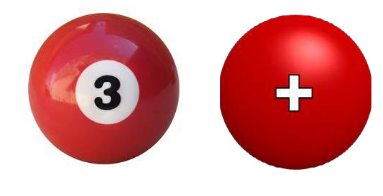
\includegraphics[width=.2\linewidth]{Quimica-Geral-Aula/bola-bilhar.png}
\end{center}


\end{Box2}

\begin{Box2}{Problemas do Modelo}
\begin{itemize}
\item Não explicou a Eletricidade nem a Radioatividade.
\end{itemize}
\end{Box2}

\section{Modelo de Thomson}
\label{sec:org16a26da}

O modelo atômico de Thomson foi proposto no ano de 1898 pelo físico inglês Joseph John Thomson ou, simplesmente, J.J. Thomson.



\begin{Box2}{Modelo do Pudim de Passas}
\begin{itemize}
\item Thomson propôs que o átomo seria uma espécie de bolha  gelatinosa,  completamente  maciça  na  qual  haveria a totalidade da carga POSITIVA homogeneamente distribuída.
\item Ele propôs que o átomo é esférico, divisível e eletricamente neutro.
\item O átomo é formado por um núcleo positivo e elétrons negativos.
\item Os elétrons estão distribuídos uniformemente ao redor do núcleo positivo.
\item Os elétrons podem ser transferidos a outros átomos, em determinadas condições.
\item Incrustada nessa gelatina estariam os Elétrons de carga NEGATIVA.
\item A Carga total do átomo seria igual a zero.
\end{itemize}
\begin{center}
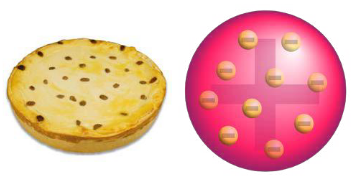
\includegraphics[width=.9\linewidth]{Quimica-Geral-Aula/pudim.png}
\end{center}

O Modelo Atômico de Thomson foi derrubado em 1908 por Ernerst Rutherford.

\end{Box2}


\subsection{A  RADIOATIVIDADE  E  A  DERRUBADA  DO MODELO DE THOMSON}
\label{sec:org61636e6}

\textbf{W. K. Röntgen} estudava raios emitidos pela ampola de Crookes. Repentinamente, notou que raios descon-hecidos saíam dessa ampola, atravessavam corpos e impressionavam chapas fotográficas. Como os raios eram desconhecidos, chamou-os de \emph{RAIOS-X}.

\textbf{Henri Becquerel} tentava relacionar fosforescência de minerais à base de urânio com os raios X. Pensou que dependiam da luz solar. Num dia nublado, guardou uma amostra de urânio numa gaveta embrulhada em papel preto e espesso. Mesmo assim, revelou uma chapa fotográfica. Iniciam-se, portanto, os estudos relacionados à \textbf{RADIOATIVIDADE}.


\subsection{CASAL CURIE E A RADIOATIVIDADE}
\label{sec:org342ab5f}


O casal Curie  – Pierre e Marie Curie – formou uma notável parceria e fez grandes descobertas, como os elementos polônio, em homenagem à terra natal de  Marie,  e  \textbf{rádio},  de  “radioatividade”,  ambos  de  importância  fundamental  no  grande  avanço  que  seus estudos imprimiram ao conhecimento da estru-tura da matéria.

\subsection{O EXPERIMENTO DE RUTHERFORD}
\label{sec:org8cd2f7c}

Ernest Rutherford, Convencido por J. J. Thomson, começa a pesquisar materiais radioativos e, aos 26 anos de idade, notou que havia dois tipos de radiação: Uma positiva (alfa) e outra negativa (beta). Assim, inicia-se o processo para determinação do NOVO MODELO ATÔMICO.

Rutherford propõe a dois de seus alunos - Johannes Hans  Wilhelm  Geiger  e  Ernerst  Marsden  -  que  bombardeassem  finas  folhas  de  metais  com  as  partículas alfa, a fim de comprovar, ou não, a validade do modelo atômico de Thomson.

\begin{center}
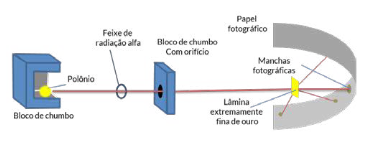
\includegraphics[width=.9\linewidth]{Quimica-Geral-Aula/placa.png}
\end{center}

Como o átomo, segundo Thomson, era uma espécie de  bolha  gelatinosa,  completamente  neutra,  no  momento em que as partículas Alfa (numa veloci-dade muito grande) colidissem com esses átomos, passariam  direto,  podendo  sofrer  pequeníssimos  desvios de sua trajetória.

Rutherford observou que: (1) a maioria das partículas alfa atravessam a lâmina de ouro sem sofrer desvios; (2) algumas partículas alfa sofreram desvios de até 90º  ao  atravessar  a  lâmina  de  ouro;  (3)  algumas  partículas alfa \textbf{RETORNARAM}.

\section{Modelo de Rutherford}
\label{sec:org59b49d4}

\begin{Box2}{Modelo Planetário}
Para que uma partícula alfa pudesse inverter sua trajetória,  deveria  encontrar  uma  carga  positiva  bastante concentrada na região central (o núcleo), com massa bastante pronunciada.

Rutherford propôs que o \textbf{NÚCLEO}, conteria toda a massa do átomo, assim como a totalidade da carga positiva (chamadas de \textbf{PRÓTONS}).

Os  elétrons  estariam  girando  circularmente  ao  redor  desse  núcleo,  numa  região  chamada  de  ELETROSFERA. Surge, assim, o \textbf{ÁTOMO NUCLEAR!}

\begin{center}
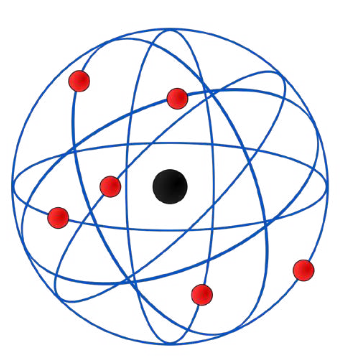
\includegraphics[scale=0.25]{./Quimica-Geral-Aula/atomo-nuclear.png}
\end{center}

\end{Box2}


\begin{Box2}{Problemas do Modelo Rutherford}
Para os físicos, toda carga elétrica em movimento, como  os  elétrons,  perde  energia  na  forma  de  luz,  diminuindo  sua  energia  cinética  e  a  consequente  atração  entre  prótons  e  elétrons  faria  com  que  houvesse  uma  colisão  entre  eles,  destruindo  o  átomo, ALGO QUE NÃO OCORRE.

Portanto, o Modelo Atômico de Rutherford, mesmo explicando o que foi observado no laboratório, apresenta uma INCORREÇÃO.
\end{Box2}

\section{Modelo de Bohr}
\label{sec:org4299274}

Niels Bohr estudava espectros de emissão do gás hidrogênio. O gás hidrogênio aprisionado numa ampola  submetida  a  alta  diferença  de  potencial  emitia luz vermelha
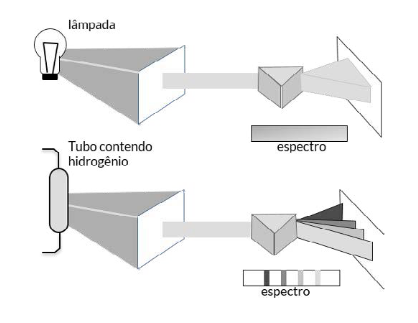
\includegraphics[scale=.5]{./Quimica-Geral-Aula/lamp.png}

Ao passar por um prisma, essa luz se subdividia em diferentes  comprimentos  de  onda  e  frequência,  caracterizando  um  ESPECTRO  LUMINOSO  DESCONTÍNUO.

\begin{Box2}{Postulados de Bohr}
\begin{enumerate}
\item A  ELETROSFERA está dividida em CAMADAS ou NÍVEIS DE ENERGIA (K, L, M, N, O, P e Q), e os elétrons nessas camadas, apresentam energia constante.  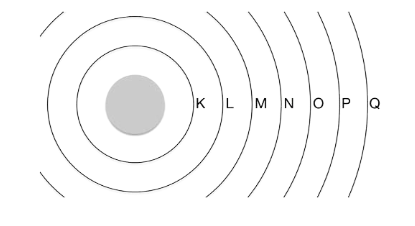
\includegraphics[scale=.3]{./Quimica-Geral-Aula/camadas.png}
\item Em sua camada de origem (camada estacionária), a  energia  é  constante,  mas  o  elétron  pode  saltar  para  uma  camada  mais  externa,  sendo  que,  para  tal, é necessário que ele ganhe energia externa.
\item Um  elétron  que  saltou  para  uma  camada  de  maior energia fica instável e tende a voltar a sua camada de origem. Nesta volta, ele devolve a mesma quantidade de energia que havia ganhado para o salto e emite um \textbf{FÓTON DE LUZ}.
\end{enumerate}

\end{Box2}
 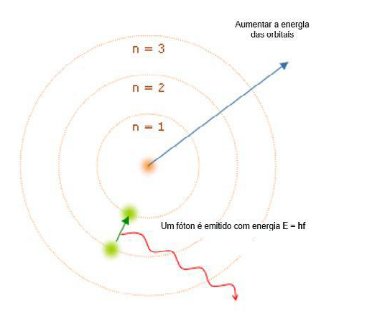
\includegraphics[scale=.5]{./Quimica-Geral-Aula/foton.png}  

O modelo atômico de Rutherford, modificado por Bohr, é também conhecido como modelo de Rutherford-Bohr.
\textbf{OBS:} O número máximo de elétrons por camadas é:  K = 2	L = 8	M = 18	N = 32	O = 32	P = 18	Q = 2.


\section{A DESCOBERTA DO NÊUTRON}
\label{sec:org3377517}

Em 1932, \textbf{James Chadwick} descobriu a partícula do núcleo atômico responsável pela sua ESTABILIDADE, que passou a ser conhecida por NÊUTRON, devido ao fato de não ter carga elétrica. Por essa descoberta ganhou o Prêmio Nobel de Física em 1935.
\begin{center}
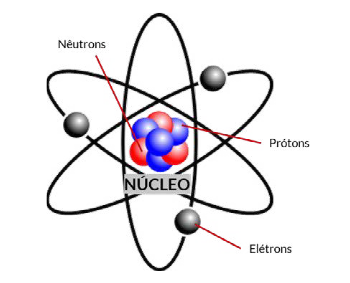
\includegraphics[width=.9\linewidth]{Quimica-Geral-Aula/atomo.png}
\end{center}

\subsection{PARTÍCULAS DO ÁTOMO}
\label{sec:org13ecce0}

\begin{itemize}
\item Os prótons têm carga elétrica positiva.
\item Os elétrons carga negativa.
\item Os nêutrons não têm carga nenhuma.
\end{itemize}
\section{Modelo atômico de Sommerfeld}
\label{sec:org5b72b75}

Arnold. J. W. Sommerfeld, em 1916, interpretou espectros com múltiplas linhas justapostas e segundo ele, as camadas enunciadas por Bohr (K, L, M, N\ldots{}) eram constituídas por subcamadas, de órbitas elípticas e de diferentes momentos angulares, conforme exibe a figura a seguir.


\begin{center}
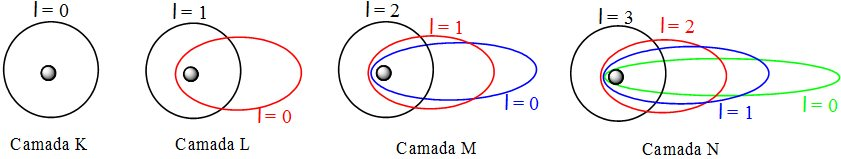
\includegraphics[width=.9\linewidth]{Quimica-Geral-Aula/modelo-atomico-sommerfeld1.png}
\end{center}


As órbitas elípticas de Sommerfeld indicaram um segundo número quântico, denominado número quântico secundário (\(l\)). Este número quântico secundário, definido pela equação \(l\) = n – 1 descreveria as subcamadas de energia e por consequência, seu momento angular. Para a camada M (n=3) teremos para o valor do número quântico secundário l = 2. Conforme se observa na figura acima, teremos para a camada M três órbitas possíveis (0, 1 e 2), sendo a órbita de maior valor a mais arredondada e onde o elétron possuirá o maior nível de energia.

A proposta de Sommerfeld conseguira, através da instituição do segundo número quântico, explicar como os espectros de emissão apresentavam o fenômeno de linhas múltiplas nas raias espectrais. Segundo este modelo, as múltiplas linhas seriam os subníveis de energia que compõem o nível ou camada de energia e estes subníveis foram caracterizados como “s”, “p”, “d” e “f”, derivados de conceitos relativos à espectroscopia.

Sommerfeld, ao manter preceitos do modelo de Bohr, determinou intacta a natureza quântica do elétron. Os subníveis de energia explicavam a existência de espectros compostos por linhas justapostas, embora ainda se mantivessem dúvidas acerca de espectros obtidos sob a ação de intensos campos magnéticos.

Sob a ação de campos magnéticos, o espectro se decompõe, exibindo novas bandas espectrais. Para explicar o surgimento destas bandas, foi proposto que o elétron reagiria ao campo magnético acumulando determinado valor de energia e isso alteraria o seu momento magnético. Tal proposição permitiu a determinação do terceiro número quântico, o número quântico magnético (\(m_l\))




\section{Modelo Atual}
\label{sec:orge9ca809}
\begin{Box2}{Nuvem Eletrônica}
Região  do  espaço  onde  há  probabilidade  de  se  encontrar um elétron com uma dada energia.
\begin{center}
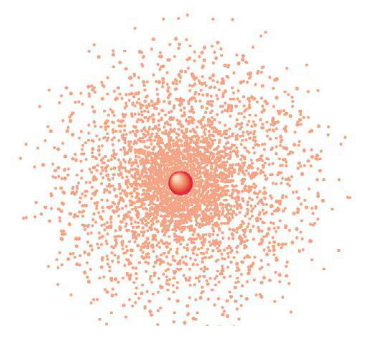
\includegraphics[scale=.4]{Quimica-Geral-Aula/nuvem.png}
\end{center}
\end{Box2}


\subsection{LOUIS DE BROGLIE}
\label{sec:org1c1c10b}

\begin{description}
\item[{DUALIDADE DA MATÉRIA:}] Toda e qualquer massa pode se comportar como onda
\end{description}


\subsection{SCHRÖDINGER}
\label{sec:orgcbcd153}

\begin{description}
\item[{ORBITAIS:}] Desenvolve o “MODELO QUÂNTICO DO ÁTOMO” ou “MODELO PROBABILÍSTICO”, colocando uma equação matemática (EQUAÇÃO DE ONDA) para o cálculo da probabilidade de encon-trar um elétron girando em uma região do espaço denominada “ORBITAL ATÔMICO”.
\end{description}
\begin{equation*}
\displaystyle\frac{\partial^2\psi}{\partial x^2} + \frac{8\pi^2m}{h^2}(E-V)\psi = 0
\end{equation*}

\subsection{HEISENBERG}
\label{sec:org5cff853}

\begin{description}
\item[{PRINCÍPIO  DA  INCERTEZA:}] É  impossível  determinar ao mesmo tempo a posição e a velocidade do elétron. Se determinarmos sua posição, não saber-emos a medida da sua velocidade e vice-versa.
\end{description}


\section{Diagrama de Linus Pauling}
\label{sec:org1c6dbe5}

Atualmente, os cientistas preferem identificar os elétrons mais por seu conteúdo de energia do que por sua posição na eletrosfera. Por meio de cálculos matemáticos, chegou-se a conclusão de que os elétrons se dispõe ao redor do núcleo atômico de acordo com sua energia.
  O cientista americano Linus Pauling (1901-1994) imaginou um diagrama (conhecido como diagrama de Pauling) onde ordenou os elétrons segundo suas energias.

Fazer uma distribuição eletrônica é definir toda a configuração da eletrosfera em estudo, determinando sua quantidade de níveis, subníveis e quantidade de elétrons em cada um desses níveis e subníveis.

\begin{tikzpicture}[x=2cm,y=2cm,scale=.5]
    \tikzset{%
            dot/.style={fill=orange!20,circle},
            gdot/.style={fill=violet!20,circle},
            set/.style={postaction={decorate,decoration={
        markings,
        mark=at position .5 with {\arrow[red]{Stealth}}
      }}}}
    \foreach\l[count=\c] in {Q,P,...,K}
    {
        \draw[dotted] (0,\c) -- (5.0, \c);
        \node at (-1.0, \c){\bfseries\l};
    }
    
    \foreach\n[count=\y] in {7,...,1}
    {
        \draw[dotted] (0,\y) -- (5.0,\y);
        \node at (-0.5,\y){\bfseries\n};
    }
    
    \foreach \x in {1,2,...,4}
    {
        \draw[dotted] (\x,0) -- (\x,8);
        \node at (\x,-0.5){\x};
    }

    %%%%% S %%%
    \node[dot] (1) at (1,7){1s};
    \node[dot] (2s) at (1,6){2s};
    \node[dot] (3s) at (1,5){3s};
    \node[dot] (4s)at (1,4){4s};
    \node[dot] (5s) at (1,3){5s};
    \node[dot] (6s) at (1,2){6s};
    \node[dot] (7s) at (1,1){7s};
    %%%%% Block p
    \node[gdot] (2p) at (2,6){2p};
    \node[gdot] (3p) at (2,5){3p};
    \node[gdot] (4p) at (2,4){4p};
    \node[gdot] (5p) at (2,3){5p};
    \node[gdot] (6p) at (2,2){6p};
    \node[gdot] (7p) at (2,1){7p};
    %\node[dot] at (2,1){};
    %%%%% Block d
    \node[dot] (3d) at (3,5){3d};
    \node[dot] (4d) at (3,4){4d};
    \node[dot] (5d) at (3,3){5d};
    \node[dot] (6d) at (3,2){6d};
    %%%%% Block f
    \node[gdot] (4f) at (4,4){4f};
    \node[gdot] (5f) at (4,3){5f};   
    
    \draw (1) edge [set,out=-135,in=45,looseness=6] (2s); 
    \draw (2s) edge [set,out=-135,in=45,looseness=5] (2p);
    \draw [red] (2p) -- (3s);
    \draw (3s) edge [set,out=-135,in=45,looseness=5] (3p); 
    \draw[red] (3p)--(4s);
    \draw (4s) edge [set,out=-135,in=45,looseness=3] (3d); 
    \draw[red] (3d)--(4p) (4p) -- (5s);
    \draw (5s) edge [set,out=-135,in=45,looseness=3] (4d);
    \draw[red] (4d)--(5p) (5p) -- (6s);
    \draw (6s) edge [set,out=-135,in=45,looseness=2.5] (4f);
    \draw[red] (4f) -- (5d) (5d) -- (6p) (6p) -- (7s);
    \draw (7s) edge [set,out=-135,in=45,looseness=2.5] (5f);
    \draw[red] (5f) -- (6d) (6d) -- (7p) (7p) edge[red,-Stealth]++ (-.5,-.5);
    
    
\end{tikzpicture}
Ordem crescente de energia dos subníveis: \emph{1s 2s 2p 3s 3p 4s 3d 4p 5s 4d 5p 6s 4f 5d 6p 7s 5f 6d 7p}


A distribuição eletrônica é feita de acordo com o número atômico (número de prótons) do elemento em questão.

 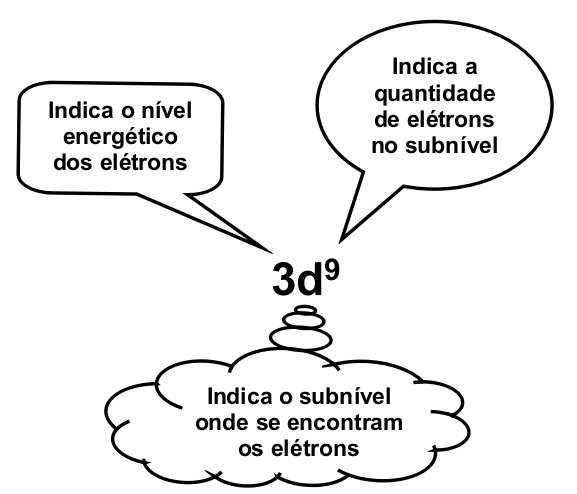
\includegraphics[scale=.3]{Quimica-Geral-Aula/subnivel.png}

A distribuição dos elétrons de um elemento por Linus Pauling nos fornece algumas informações :

\begin{enumerate}
\item A que período pertence o elemento = nível mais alto da distribuição.
\item O número de elétrons da última camada = soma dos elétrons do último nível.
\item A localização do elétron mais periférico = é o elétron que se encontra na última camada da distribuição.
\item O elétron mais energético é o último elétron da distribuição.
\item A que tipo de família pertence o elemento :
\begin{itemize}
\item Se a distribuição terminar em s ou p, o elemento pertence à família 1-2 ou 13-18 .
\item Se a distribuição terminar em d ou f, o elemento pertence à família 3-12 .
\end{itemize}
\item O número da família a que pertence o elemento :
\begin{description}
\item[{s}] = o expoente indica o número da família 1.
\item[{p}] = a soma do último s e p mais dez (10), indica o número da família 1-2 e 13-18.
\item[{d}] = a soma do último s e d indica o número da família 3-12.
\item[{f}] = são os elementos de transição interna e pertencem à família 3 do sexto e sétimo
\end{description}
\end{enumerate}
período.

\begin{Box2}{Exemplo}
 \ch{^{51}Sb}

 \(1s^2 – 2s^2 – 2p^6 – 3s^2 – 3 p^6 – 4 s^2 – 3 d^{10} – 4 p^6 – 5 s^2 – 4 d^{10} – 5 p^3\) 
\end{Box2}

\textbf{\ch{5 p^3}} – É o último da distribuição. Isso quer dizer que o elétron mais energético se encontra no subnível p, do quinto nível. O elétron mais periférico coincide com o mais energético, pois ele também representa a última camada.
O elemento pertence ao  \ang{5} período e à família 15 (5A) pois a soma do último s, d e p dá um valor igual a 15 .

\section{Identificação do átomo}
\label{sec:org6924b51}

Os átomos são identificados segundo o seu número de prótons, nêutrons e elétrons. Assim, convém sabermos alguns conceitos:

\textbf{Número atômico (Z)} – É a quantidade de prótons existente no núcleo do átomo.

\textbf{Número de nêutrons (N)} – É a quantidade de nêutrons existentes no núcleo do átomo.

\textbf{Número de massa (A)} – É a soma dos números de prótons e nêutrons existentes no núcleo atômico.

\begin{center}
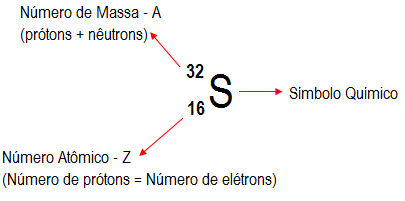
\includegraphics[width=.9\linewidth]{Quimica-Geral-Aula/iso.png}
\end{center}

Em um \textbf{átomo neutro} o número de prótons é igual ao número de elétrons. Um átomo que apresenta o seu número de elétrons diferente do número de prótons é um \textbf{íon}. Um íon positivo é conhecido pelo nome de \textbf{cátion} e apresenta número de elétrons menor do que o número de prótons (perda de elétrons). Um íon negativo é conhecido pelo nome de \textbf{ânion} e apresenta número de elétrons maior do que o número de prótons (ganho de elétrons)

\section{Números Quânticos}
\label{sec:org46a18c5}

\subsection{Número quântico principal}
\label{sec:org2842631}

O número quântico principal (n) define o nível de energia ou a camada que os elétrons possuem, definindo também a distância do orbital em relação ao núcleo e o tamanho do orbital ocupado pelo elétron. Tal conceito se assemelha ao conceito de camada, adotado por Niels Böhr e pode ser assim exemplificado:
\begin{center}
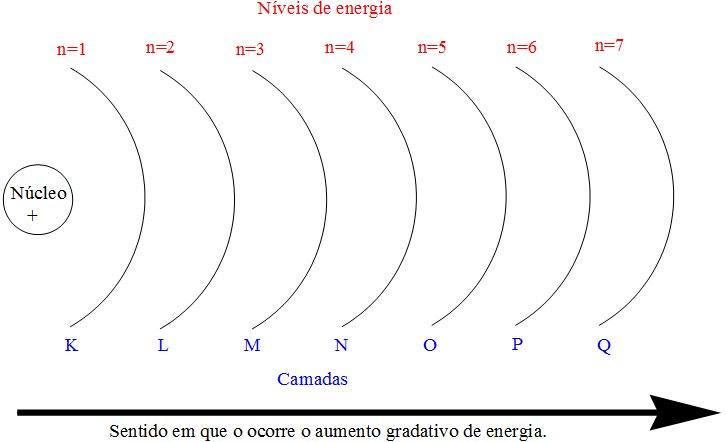
\includegraphics[scale=.3]{Quimica-Geral-Aula/niveis-de-energia.jpg}
\end{center}

\subsection{Número quântico de momento angular (\(l\))}
\label{sec:orgecdc9a7}

O número quântico secundário, azimutal ou de momento angular (\(l\)) é aquele que indica os subníveis de energia, ou seja, o subnível energético a que o elétron pertence.

\begin{tblr}{|c|c|c|c|}
\hline
$l$ & 0 & 1 & 2 & 3 \\ \hline
Orbital & s & p & d & f\\ \hline
\end{tblr}


\subsection{Número quântico magnético (m\textsubscript{l})}
\label{sec:org8958f1a}

O número quântico magnético (m ou \(m_l\)) é aquele que indica os orbitais no espaço onde os elétrons se encontram, ou seja, a região mais provável de encontrar um elétron dentro de um subnível de energia.
\begin{center}
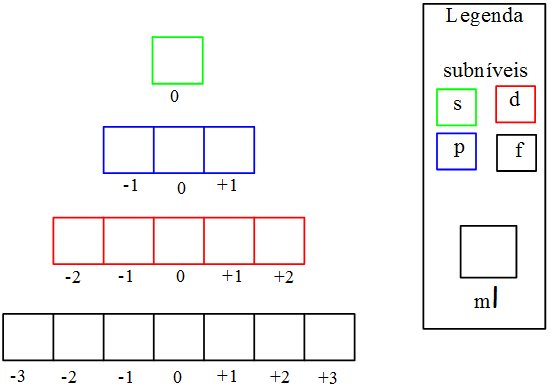
\includegraphics[scale=.4]{Quimica-Geral-Aula/numero-quantico-magnetico.jpg}
\end{center}

\subsection{Número quântico spin (m\textsubscript{s})}
\label{sec:org12a0ca6}

O número quântico Spin (S ou \(m_s\)) caracteriza o possível movimento rotacional dos elétrons, sob seus eixos imaginários.
\begin{center}
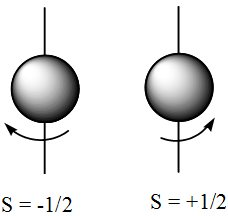
\includegraphics[scale=.4]{Quimica-Geral-Aula/numero-quantico-spin.jpg}
\end{center}




\begin{figure*}

\section{Material Apoio}
\label{sec:orgdc8c459}


\begin{center}
\begin{talltblr}{lll}
\textbf{Conteúdo} & \textbf{Aula} & \textbf{Scan}\\[0pt]
Modelos Atômicos Dalton e Thompson & \url{https://youtu.be/l5C1qq37W48} & \qrcode[height=1.6cm]{https://youtu.be/l5C1qq37W48}\\[0pt]
 &  & \\[0pt]
Modelo de Bohr & \url{https://youtu.be/-1tQAFJyxho} &  \qrcode[height=1.6cm]{https://youtu.be/-1tQAFJyxho}\\[0pt]
 &  & \\[0pt]
Tabela Periódica & \url{https://youtu.be/yv5168bi1X4} &  \qrcode[height=1.6cm]{https://youtu.be/yv5168bi1X4}\\[0pt]
 &  & \\[0pt]
Distribuição Eletrônica & \url{https://youtu.be/LYhckRAtCPU} &  \qrcode[height=1.6cm]{https://youtu.be/LYhckRAtCPU}\\[0pt]
 &  & \\[0pt]
Propriedades Periódicas & \url{https://youtu.be/eaGqKb22\_7I} &  \qrcode[height=1.6cm]{https://youtu.be/eaGqKb22_7I}\\[0pt]
\end{talltblr}
\end{center}

\end{figure*}
\end{document}
